\documentclass[12pt,a4paper,oneside]{book}

\usepackage[utf8]{inputenc}
\usepackage[T1]{fontenc}
\usepackage{lmodern}
\usepackage{graphicx}
\usepackage{float}
\usepackage{amsmath,amssymb}
\usepackage{geometry}
\usepackage{hyperref}
\usepackage{xcolor}
\usepackage{listings}
\usepackage{microtype}
\usepackage{tikz}
\usetikzlibrary{arrows.meta,positioning,shapes.geometric,fit,calc}

\geometry{margin=1in}
\hypersetup{colorlinks=true,linkcolor=blue!50!black,urlcolor=blue!60!black}
\definecolor{codebg}{RGB}{247,248,250}
\definecolor{codeblue}{RGB}{38,80,150}
\lstset{language=C++,basicstyle=\ttfamily\small,keywordstyle=\color{codeblue}\bfseries,
  commentstyle=\color{gray!80!black},stringstyle=\color{green!35!black},
  numbers=left,numberstyle=\tiny\color{gray},stepnumber=1,numbersep=8pt,
  backgroundcolor=\color{codebg},frame=single,rulecolor=\color{gray!30},
  breaklines=true,showstringspaces=false,tabsize=4,columns=fullflexible,
  captionpos=b}

\makeatletter
\newcommand{\chapterauthor}[1]{%
  {\parindent0pt\vspace*{-15pt}%
  \linespread{1.1}\large\itshape\begin{flushright}#1\end{flushright}%
  \par\nobreak\vspace*{25pt}}
  \@afterheading%
}
\makeatother

\tikzset{
  uml/.style={draw=blue!55!black,rounded corners=2pt,fill=blue!4,
    align=center,minimum height=8mm,text width=31mm,font=\small},
  flow/.style={draw=blue!55!black,rounded corners=3pt,fill=blue!4,
    align=center,text width=41mm,minimum height=8mm,font=\small},
  decision/.style={diamond,draw=blue!55!black,fill=orange!10,aspect=2.1,
    align=center,inner sep=1.5pt,font=\small},
  actor/.style={draw=purple!65!black,rounded corners=3pt,fill=purple!5,
    align=center,text width=27mm,minimum height=9mm,font=\small},
  edge/.style={-{Stealth[length=2mm]},thick,draw=blue!65!black}
}

\usetikzlibrary{shapes.multipart}
\setlength{\fboxsep}{0pt}
\tikzset{
  cls/.style={rectangle split,rectangle split parts=3,draw=blue!55!black,fill=blue!4,
    font=\small,align=center,inner sep=3pt},
  cls2/.style={rectangle split,rectangle split parts=2,draw=blue!55!black,fill=blue!4,
    font=\small,align=center,inner sep=3pt},
  ucase/.style={ellipse,draw=blue!55!black,fill=blue!4,font=\small,align=center,
    text width=54mm,inner sep=1pt,minimum height=10mm},
  comp/.style={draw=blue!55!black,fill=blue!4,font=\small,align=center,
    text width=31mm,minimum height=14mm,inner sep=2pt},
  state/.style={draw=blue!55!black,fill=blue!4,rounded corners=4mm,font=\small,
    align=center,text width=24mm,minimum height=13mm,inner sep=2pt},
  art/.style={draw=blue!55!black,fill=white,font=\small,align=center,
    text width=38mm,minimum height=10mm,inner sep=2pt},
  lbl/.style={font=\scriptsize,align=center}
}
\newcommand{\umlactor}[3]{\begin{scope}[shift={(#1,#2)},purple!65!black,thick]
  \draw (0,0.6) circle (0.2);
  \draw (0,0.4)--(0,-0.1) (-0.3,0.25)--(0.3,0.25) (0,-0.1)--(-0.25,-0.55) (0,-0.1)--(0.25,-0.55);
  \node[font=\small,below,text=black] at (0,-0.55) {#3};
\end{scope}}
\newcommand{\msg}[4]{\draw[edge] (#2,#1) -- node[above,lbl,text width=37mm]{#4} (#3,#1);}
\newcommand{\ret}[4]{\draw[edge,dashed] (#2,#1) -- node[above,lbl,text width=37mm]{#4} (#3,#1);}
\newcommand{\selfmsg}[3]{\draw[edge] (#2,#1) -- ++(0.6,0) -- ++(0,-0.5) -- ++(-0.6,0);\node[lbl,anchor=west,align=left] at (#2+0.7,#1-0.25) {#3};}

\begin{document}
\mainmatter

% C++ OOP mini-project report based on the supplied chapter template.
\chapter{Online Examination System}
\chapterauthor{Kaushika M (231131)\\Neekha Zehra (251137)}

\section{Introduction and Problem Statement}
The Online Examination System, presented in the web interface as \emph{ExamEra}, is a C++ application for delivering and managing objective examinations. It provides separate student and administrator experiences. Students can register or sign in, view available examinations, take a timed attempt, submit answers, and review recorded results. Administrators can create examinations, maintain multiple-choice and true/false questions, and inspect participation and scores.

The problem addressed is the effort and delay involved in organizing timed assessments and calculating results manually. The application brings exam metadata, questions, timing, answer evaluation, and result storage into one flow. The repository includes both a console entry point and an HTTP server that serves a static HTML/CSS/JavaScript frontend and a JSON API. Persistent records are stored in plain-text files under \texttt{data/}.

This report describes the implementation present in the supplied project archive. The included screenshots show the ExamEra role-selection page, student dashboard, and administrator examination overview. Sample counts and scores visible in the screenshots are demonstration data and are not treated as performance measurements.

\section{Scope and Feature Set}
\begin{itemize}
    \item \textbf{Role-based entry:} Student registration and login use the student repository; the server also exposes an administrator login. The sample administrator account is initialized in the server source for demonstration.
    \item \textbf{Examination management:} Administrators can create examinations with a title, duration, and planned question count, then review questions and student results.
    \item \textbf{Question authoring:} The service layer supports four-option MCQs and true/false questions, validates submitted values, and supports question deletion.
    \item \textbf{Timed student attempts:} Students can see available examinations and begin an attempt. The server records an attempt start time, enforces the exam duration with a short network grace period, and rejects duplicate completed attempts.
    \item \textbf{Automatic evaluation:} The application awards each question's marks for a correct answer and zero for incorrect or unanswered questions. It computes score, percentage, grade, pass status, and attempt counts.
    \item \textbf{Result and review:} Submitted results are saved and can be listed by student or examination. The submit response includes a per-question review.
    \item \textbf{File persistence:} Students, examinations, questions, and results are read from and written to CSV-like text files in \texttt{data/}.
    \item \textbf{Browser interface:} Static pages provide role selection, login/registration, student examination and result views, and administrator management screens.
\end{itemize}

The current implementation is a small academic demonstration. It does not include a relational database, a production deployment configuration, or a question type beyond MCQ and true/false in the API. The console entry point has its own interaction flow; the screenshots correspond to the web frontend.

\section{Object-Oriented Architecture}
The application separates domain objects, application services, persistence repositories, and the HTTP presentation boundary. \texttt{main.cpp} starts the console flow; \texttt{server\_main.cpp} starts the web server. \texttt{ApiServer} routes requests and serves the static frontend. Model classes represent users, exams, question variants, answers, and results. Services coordinate authentication, question management, attempt evaluation, and exam sessions. Repository classes encapsulate text-file storage.

\begin{figure}[htbp]
\centering
\hyphenpenalty=10000 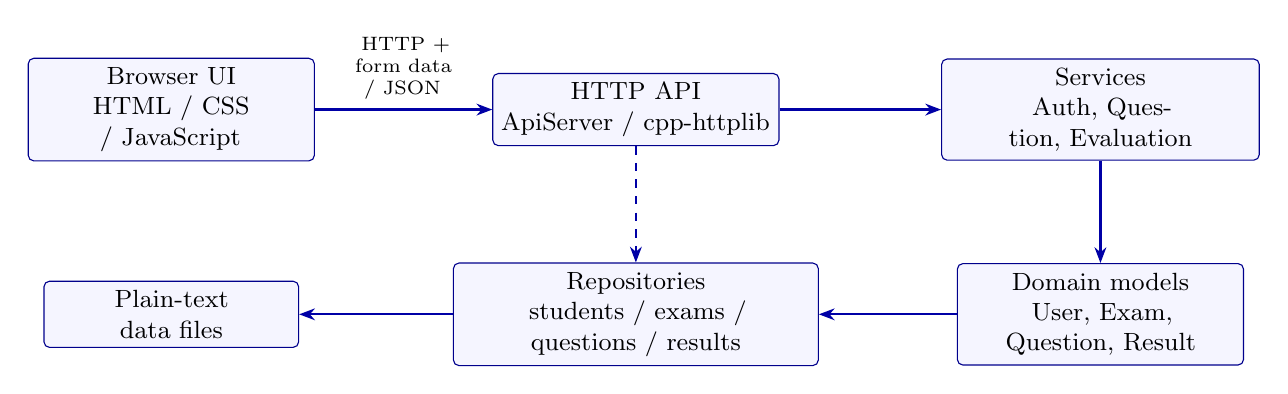
\begin{tikzpicture}
  \node[uml,text width=34mm] (ui) at (0,0) {Browser UI\\HTML / CSS / JavaScript};
  \node[uml,text width=34mm] (api) at (5.9,0) {HTTP API\\ApiServer / cpp-httplib};
  \node[uml,text width=38mm] (svc) at (11.8,0) {Services\\Auth, Question, Evaluation};
  \node[uml,text width=34mm] (model) at (11.8,-2.6) {Domain models\\User, Exam, Question, Result};
  \node[uml,text width=44mm] (repo) at (5.9,-2.6) {Repositories\\students / exams / questions / results};
  \node[uml,text width=30mm] (files) at (0,-2.6) {Plain-text\\data files};
  \draw[edge] (ui) -- node[above,lbl,text width=17mm]{HTTP + form data / JSON} (api);
  \draw[edge] (api) -- (svc);
  \draw[edge] (svc) -- (model);
  \draw[edge] (model) -- (repo);
  \draw[edge] (repo) -- (files);
  \draw[edge,dashed] (api.south) -- (repo.north);
\end{tikzpicture}
\caption{Layered view of the web execution path in the supplied implementation.}
\label{fig:architecture}
\end{figure}

\subsection{Class Design and Associations}
\texttt{User} is an abstract base class. \texttt{Student} and \texttt{Admin} inherit its identity and authentication behavior and override the role display operation. A second polymorphic hierarchy is formed by abstract \texttt{Question} and concrete \texttt{MCQQuestion} and \texttt{TrueFalseQuestion}. The question service and repository return owning \texttt{unique\_ptr<Question>} values, allowing evaluation to operate on different question types through the base interface.

An \texttt{Exam} is associated with its questions by an exam identifier. \texttt{AnswerSheet} stores answers keyed by question identifier. \texttt{EvaluationService} uses an exam, its question collection, and an answer sheet to produce a \texttt{Result}. Repositories are used by services to load and save records. The implementation does not model a persistent \texttt{QuestionPaper} containing question objects; the \texttt{QuestionPaper} value is used for descriptive exam-paper details in the console flow.

\begin{figure}[htbp]
\centering
\hyphenpenalty=10000 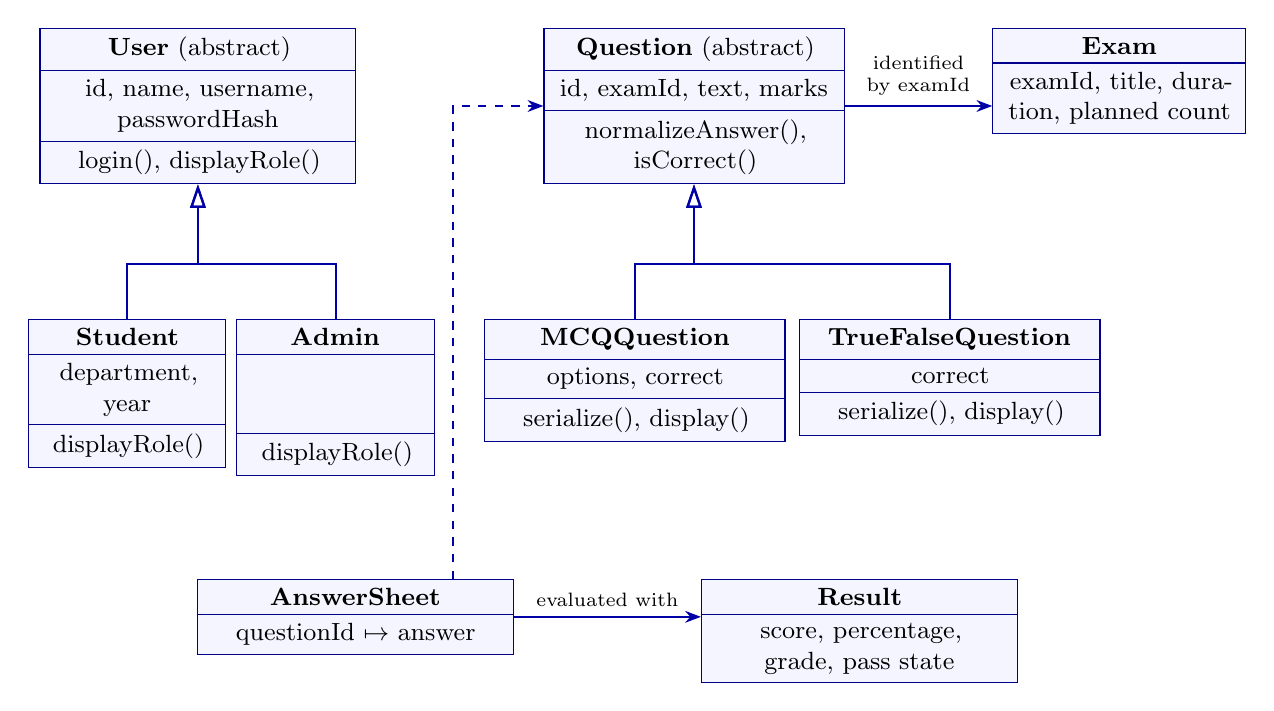
\begin{tikzpicture}
  \node[cls,anchor=north,text width=38mm] (user) at (2.2,0) {\textbf{User} (abstract)\nodepart{second}id, name, username, passwordHash\nodepart{third}login(), displayRole()};
  \node[cls,anchor=north,text width=36mm] (question) at (8.5,0) {\textbf{Question} (abstract)\nodepart{second}id, examId, text, marks\nodepart{third}normalizeAnswer(), isCorrect()};
  \node[cls2,anchor=north,text width=30mm] (exam) at (13.9,0) {\textbf{Exam}\nodepart{second}examId, title, duration, planned count};

  \node[cls,anchor=north,text width=23mm] (student) at (1.3,-3.7) {\textbf{Student}\nodepart{second}department, year\nodepart{third}displayRole()};
  \node[cls,anchor=north,text width=23mm] (admin) at (3.95,-3.7) {\textbf{Admin}\nodepart{second}\strut\\\strut\nodepart{third}displayRole()};
  \node[cls,anchor=north,text width=36mm] (mcq) at (7.75,-3.7) {\textbf{MCQQuestion}\nodepart{second}options, correct\nodepart{third}serialize(), display()};
  \node[cls,anchor=north,text width=36mm] (tf) at (11.75,-3.7) {\textbf{TrueFalseQuestion}\nodepart{second}correct\nodepart{third}serialize(), display()};

  \node[cls2,anchor=north,text width=38mm] (answer) at (4.2,-7.0) {\textbf{AnswerSheet}\nodepart{second}questionId $\mapsto$ answer};
  \node[cls2,anchor=north,text width=38mm] (result) at (10.6,-7.0) {\textbf{Result}\nodepart{second}score, percentage, grade, pass state};

  \draw[edge,-{Triangle[open,length=3mm]}] (student.north) -- ++(0,0.7) -| (user.south);
  \draw[edge,-{Triangle[open,length=3mm]}] (admin.north) -- ++(0,0.7) -| (user.south);
  \draw[edge,-{Triangle[open,length=3mm]}] (mcq.north) -- ++(0,0.7) -| (question.south);
  \draw[edge,-{Triangle[open,length=3mm]}] (tf.north) -- ++(0,0.7) -| (question.south);

  \draw[edge] (question.east) -- node[above,lbl,text width=15mm]{identified by examId} (exam.west |- question.east);
  \draw[edge] (answer.east) -- node[above,lbl]{evaluated with} (result.west |- answer.east);
  \draw[edge,dashed] (answer.north west) ++(3.25,0) coordinate (a) -- (a |- question.west) -- (question.west);
\end{tikzpicture}
\caption{Simplified domain class diagram; repository and service classes are omitted for readability.}
\label{fig:classes}
\end{figure}

\subsection{OOP Principles in the Implementation}
\textbf{Encapsulation} is used to keep state inside domain classes and expose operations through methods. For example, \texttt{AnswerSheet} owns a map of question identifiers to normalized answers, and \texttt{Result} exposes score and pass calculations through member functions.

\textbf{Abstraction and polymorphism} are visible in the pure virtual operations of \texttt{Question}. The evaluator invokes the common answer-checking interface while each concrete question type supplies its own normalization and correct answer behavior. \texttt{User} similarly defines the common role interface.

\textbf{Inheritance} is used by the student/admin roles and by concrete question types. \textbf{Composition/ownership} is expressed in collections of \texttt{unique\_ptr<Question>} returned by the question repository/service; the owning collection manages the lifetime of each concrete question. Repositories and services are separate collaborating objects rather than base-class relationships.

\begin{lstlisting}[caption={Abstract question interface and runtime-polymorphic question types (excerpt from include/models/Question.h).},label={lst:question}]
class Question {
public:
    virtual ~Question() = default;
    virtual std::string normalizeAnswer(
        const std::string& input) const = 0;
    virtual std::string getCorrectAnswer() const = 0;
    virtual std::string getType() const = 0;
    virtual void display(int number) const = 0;
    bool isCorrect(const std::string& answer) const;
};

class MCQQuestion : public Question {
public:
    std::string normalizeAnswer(
        const std::string& input) const override;
    std::string getCorrectAnswer() const override;
    // Other MCQ-specific operations...
};
\end{lstlisting}

\begin{lstlisting}[caption={Evaluation accumulates marks through the base-class interface (excerpt from src/services/EvaluationService.cpp).},label={lst:evaluation}]
for (size_t i = 0; i < questions.size(); ++i) {
    const Question& q = *questions[i];
    totalMarks += q.getMarks();

    if (!answers.hasAnswer(q.getId()))
        continue;

    ++attempted;
    if (q.isCorrect(answers.getAnswer(q.getId()))) {
        ++correct;
        score += q.getMarks();
    }
}
\end{lstlisting}

\section{System Design and UML Diagrams}
All UML diagrams in this report---use-case, class, sequence, and activity---are constructed directly in LaTeX with the TikZ package. No diagram screenshots or externally generated UML images are used. The diagrams are editable as TikZ source in this document. Reference documentation: \href{https://tikz.dev/}{Official TikZ documentation} and \href{https://www.overleaf.com/learn/latex/TikZ_package}{Overleaf TikZ package tutorial}.

\subsection{Use-Case Diagram}
Figure~\ref{fig:usecase} summarizes the visible student and administrator capabilities exposed by the web application. Authentication is required for role-specific API operations.

\begin{figure}[H]
\centering
\hyphenpenalty=10000 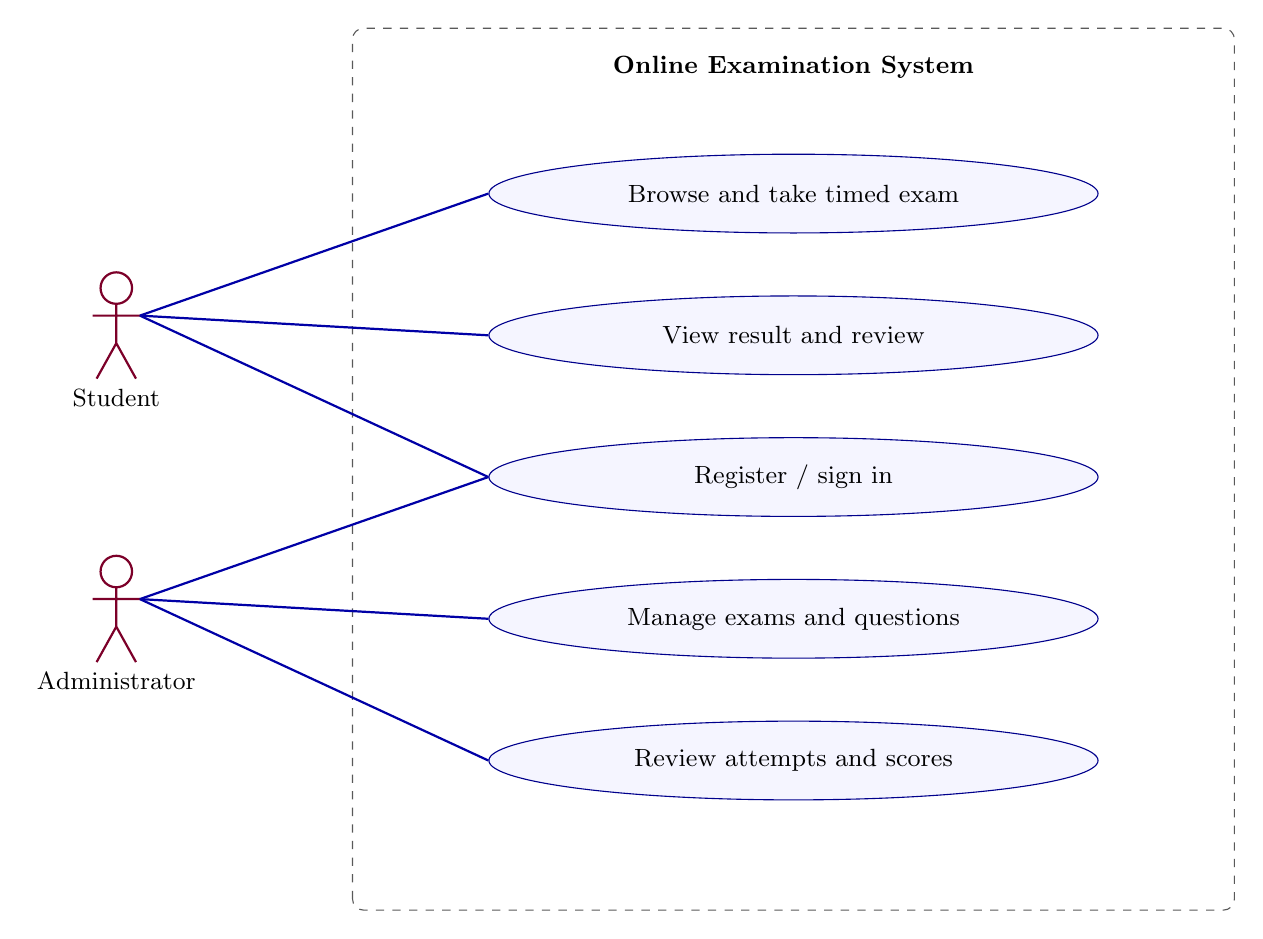
\begin{tikzpicture}
  \draw[dashed,rounded corners,gray!70!black] (4.2,-5.5) rectangle (15.4,5.7);
  \node[font=\small\bfseries] at (9.8,5.2) {Online Examination System};
  \node[ucase] (take) at (9.8,3.6) {Browse and take timed exam};
  \node[ucase] (result) at (9.8,1.8) {View result and review};
  \node[ucase] (reg) at (9.8,0) {Register / sign in};
  \node[ucase] (manage) at (9.8,-1.8) {Manage exams and questions};
  \node[ucase] (reports) at (9.8,-3.6) {Review attempts and scores};
  \umlactor{1.2}{1.8}{Student}
  \umlactor{1.2}{-1.8}{Administrator}
  \draw[thick,blue!65!black] (1.5,2.05) -- (take.west);
  \draw[thick,blue!65!black] (1.5,2.05) -- (result.west);
  \draw[thick,blue!65!black] (1.5,2.05) -- (reg.west);
  \draw[thick,blue!65!black] (1.5,-1.55) -- (reg.west);
  \draw[thick,blue!65!black] (1.5,-1.55) -- (manage.west);
  \draw[thick,blue!65!black] (1.5,-1.55) -- (reports.west);
\end{tikzpicture}
\caption{Use cases supported by the web interface and API.}
\label{fig:usecase}
\end{figure}

\subsection{Sequence Diagram: Student Exam Attempt}
The server-side start endpoint verifies the student session and eligibility, records a start time, and returns the exam and questions. On submission it normalizes answers, evaluates them, saves the result, and returns result and review data.

\begin{figure}[H]
\centering
\hyphenpenalty=10000 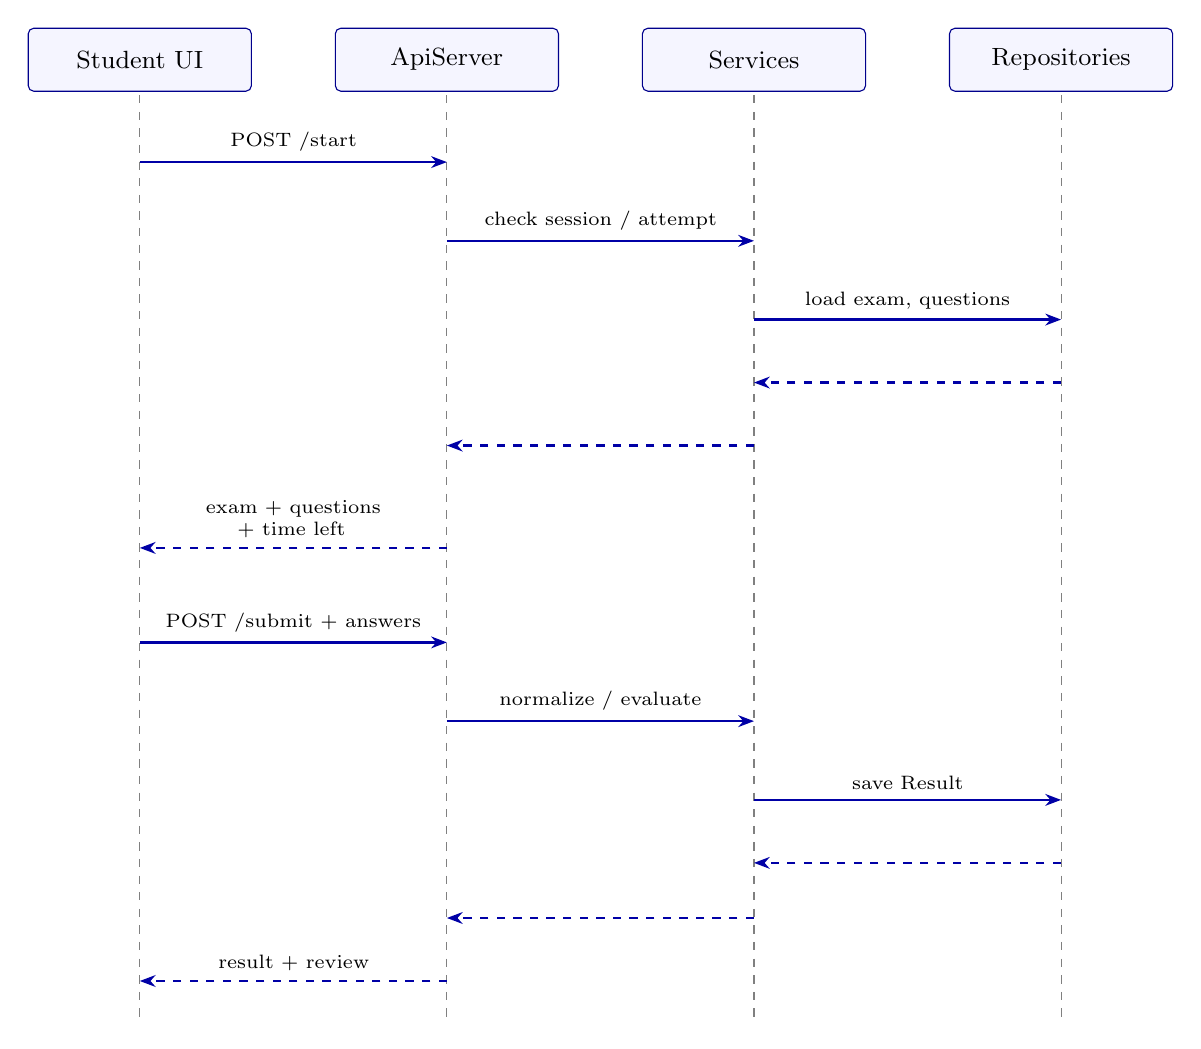
\begin{tikzpicture}
  \foreach \x/\t in {1.3/Student UI,5.2/ApiServer,9.1/Services,13.0/Repositories}{
    \node[uml,text width=26mm] at (\x,0) {\t};
    \draw[dashed,gray] (\x,-0.45) -- (\x,-12.2);}
  \msg{-1.3}{1.3}{5.2}{POST /start}
  \msg{-2.3}{5.2}{9.1}{check session / attempt}
  \msg{-3.3}{9.1}{13.0}{load exam, questions}
  \ret{-4.1}{13.0}{9.1}{}
  \ret{-4.9}{9.1}{5.2}{}
  \ret{-6.2}{5.2}{1.3}{exam + questions\\+ time left}
  \msg{-7.4}{1.3}{5.2}{POST /submit + answers}
  \msg{-8.4}{5.2}{9.1}{normalize / evaluate}
  \msg{-9.4}{9.1}{13.0}{save Result}
  \ret{-10.2}{13.0}{9.1}{}
  \ret{-10.9}{9.1}{5.2}{}
  \ret{-11.7}{5.2}{1.3}{result + review}
  \end{tikzpicture}
\caption{Representative server-backed student attempt sequence.}
\label{fig:sequence}
\end{figure}

\subsection{Activity Diagram: Attempt and Evaluation}
\begin{figure}[H]
\centering
\hyphenpenalty=10000 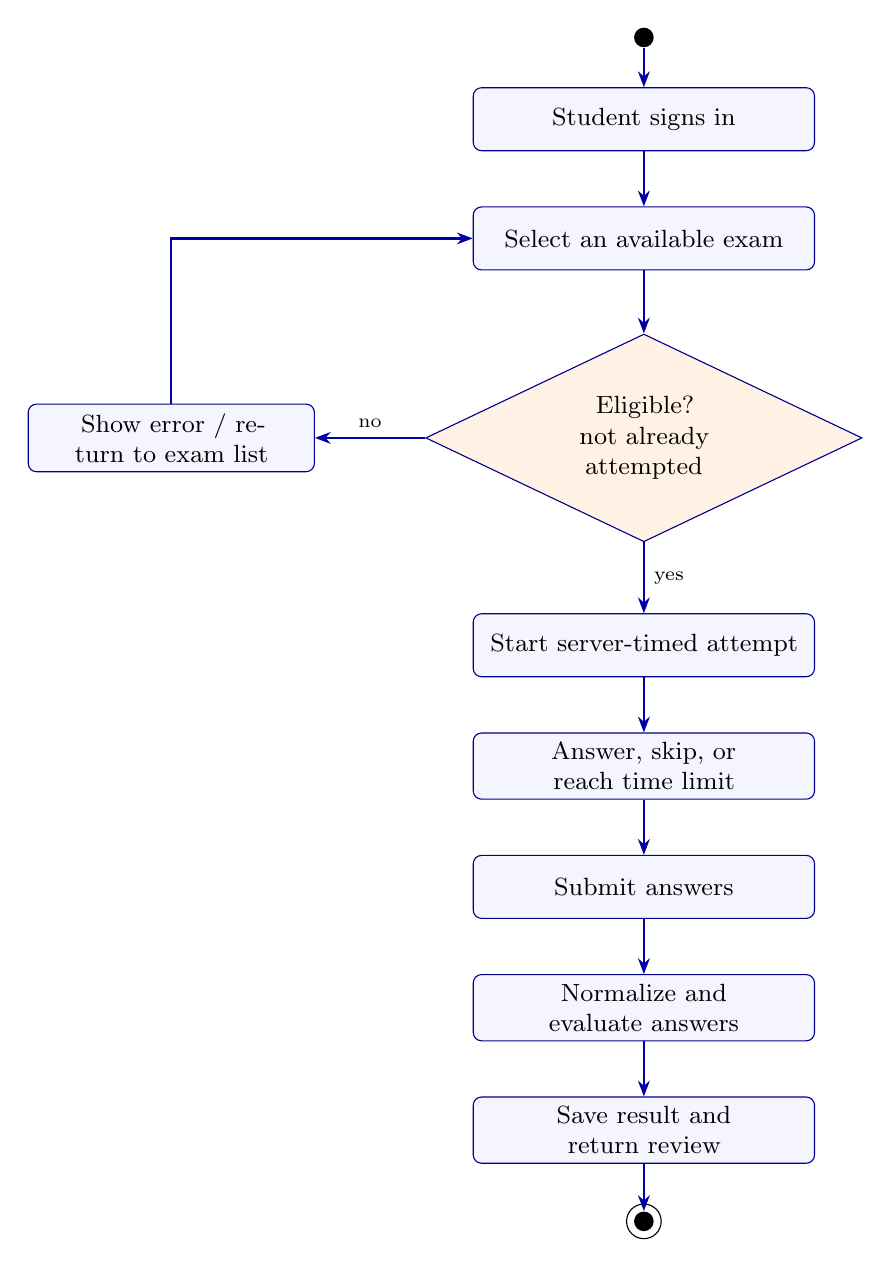
\begin{tikzpicture}[node distance=7mm]
  \node[circle,fill=black,inner sep=2.5pt] (init) at (0,0) {};
  \node[flow,below=5mm of init] (login) {Student signs in};
  \node[flow,below=of login] (select) {Select an available exam};
  \node[decision,below=8mm of select,text width=30mm] (eligible) {Eligible?\\not already attempted};
  \node[flow,left=14mm of eligible,text width=34mm] (reject) {Show error / return to exam list};
  \node[flow,below=9mm of eligible] (start) {Start server-timed attempt};
  \node[flow,below=of start] (answer) {Answer, skip, or reach time limit};
  \node[flow,below=of answer] (submit) {Submit answers};
  \node[flow,below=of submit] (evaluate) {Normalize and evaluate answers};
  \node[flow,below=of evaluate] (persist) {Save result and return review};
  \node[circle,fill=black,inner sep=2.5pt,below=6mm of persist] (end) {};
  \draw (end) circle (2.2mm);
  \draw[edge] (init) -- (login);
  \draw[edge] (login) -- (select);
  \draw[edge] (select) -- (eligible);
  \draw[edge] (eligible) -- node[right,lbl]{yes} (start);
  \draw[edge] (eligible) -- node[above,lbl]{no} (reject);
  \draw[edge] (reject.north) |- (select.west);
  \draw[edge] (start) -- (answer);
  \draw[edge] (answer) -- (submit);
  \draw[edge] (submit) -- (evaluate);
  \draw[edge] (evaluate) -- (persist);
  \draw[edge] (persist) -- (end);
\end{tikzpicture}
\caption{Student attempt activity, including the duplicate-attempt guard.}
\label{fig:activity}
\end{figure}

\subsection{State Diagram: Student Attempt Lifecycle}
Figure~\ref{fig:state} shows the states an examination passes through for one student.

\begin{figure}[H]
\centering
\hyphenpenalty=10000 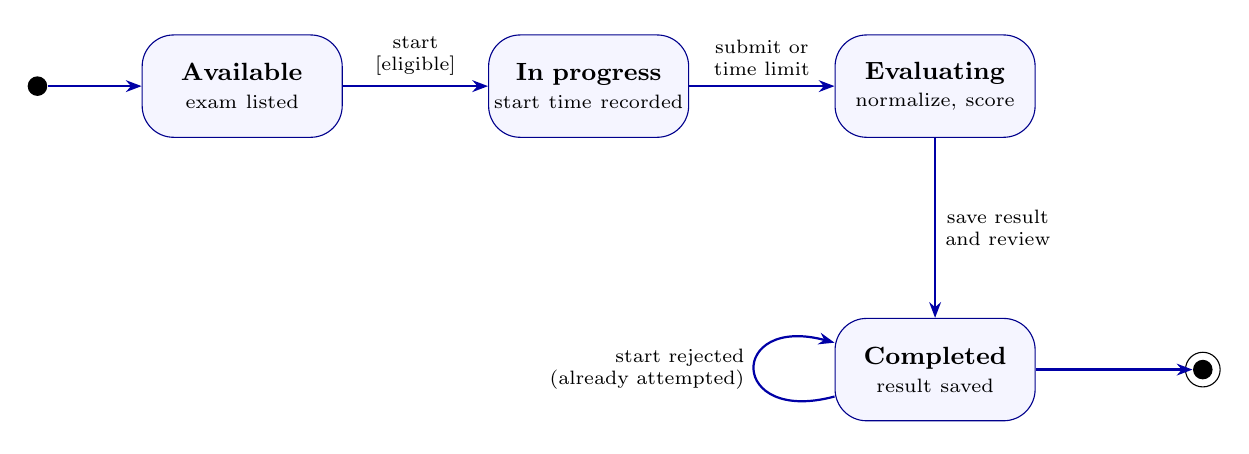
\begin{tikzpicture}
  \node[circle,fill=black,inner sep=2.5pt] (init) at (0,0) {};
  \node[state] (avail) at (2.6,0) {\textbf{Available}\\[-1pt]\scriptsize exam listed};
  \node[state] (prog) at (7.0,0) {\textbf{In progress}\\[-1pt]\scriptsize start time recorded};
  \node[state] (eval) at (11.4,0) {\textbf{Evaluating}\\[-1pt]\scriptsize normalize, score};
  \node[state] (done) at (11.4,-3.6) {\textbf{Completed}\\[-1pt]\scriptsize result saved};
  \node[circle,fill=black,inner sep=2.5pt] (fin) at (14.8,-3.6) {};
  \draw (fin) circle (2.2mm);
  \draw[edge] (init) -- (avail);
  \draw[edge] (avail) -- node[above,lbl]{start\\{[}eligible{]}} (prog);
  \draw[edge] (prog) -- node[above,lbl]{submit or\\time limit} (eval);
  \draw[edge] (eval) -- node[right,lbl]{save result\\and review} (done);
  \draw[edge] (done) -- (fin);
  \path (done) edge[edge,loop left,min distance=14mm] node[left,lbl,align=right]{start rejected\\(already attempted)} (done);
\end{tikzpicture}
\caption{States of an examination for one student, including rejection of a duplicate attempt.}
\label{fig:state}
\end{figure}

\subsection{Component Diagram}
Figure~\ref{fig:component} groups the implementation into deployable components and their dependencies.

\begin{figure}[H]
\centering
\hyphenpenalty=10000 \begin{tikzpicture}
  \node[comp] (ui) at (1.8,0) {\scriptsize\guillemotleft component\guillemotright\\\textbf{Browser frontend}\\HTML / CSS / JS};
  \node[comp] (api) at (7.6,0) {\scriptsize\guillemotleft component\guillemotright\\\textbf{ApiServer}\\cpp-httplib routes};
  \node[comp] (auth) at (1.8,-3.2) {\scriptsize\guillemotleft component\guillemotright\\\textbf{Authentication service}};
  \node[comp] (sess) at (5.9,-3.2) {\scriptsize\guillemotleft component\guillemotright\\\textbf{Exam session}};
  \node[comp] (qsvc) at (10.0,-3.2) {\scriptsize\guillemotleft component\guillemotright\\\textbf{Question service}};
  \node[comp] (eval) at (14.1,-3.2) {\scriptsize\guillemotleft component\guillemotright\\\textbf{Evaluation service}};
  \node[comp] (r1) at (1.8,-6.2) {\textbf{Student}\\repository};
  \node[comp] (r2) at (5.9,-6.2) {\textbf{Exam}\\repository};
  \node[comp] (r3) at (10.0,-6.2) {\textbf{Question}\\repository};
  \node[comp] (r4) at (14.1,-6.2) {\textbf{Result}\\repository};
  \node[comp,text width=140mm,minimum height=9mm] (files) at (7.95,-8.9) {\textbf{Plain-text data files} (\texttt{data/})};
  \draw[edge,dashed] (ui) -- node[above,lbl]{HTTP / JSON} (api);
  \foreach \c in {auth,sess,qsvc,eval} \draw[edge,dashed] (api.south) -- ++(0,-0.65) -| (\c.north);
  \foreach \a/\b in {auth/r1,sess/r2,qsvc/r3,eval/r4} \draw[edge,dashed] (\a) -- (\b);
  \foreach \r in {r1,r2,r3,r4} \draw[edge,dashed] (\r.south) -- (\r.south |- files.north);
\end{tikzpicture}
\caption{Component view of the web application and its persistence layer.}
\label{fig:component}
\end{figure}

\subsection{Deployment Diagram}
Figure~\ref{fig:deployment} shows how the web and console executables relate to the data files.

\begin{figure}[H]
\centering
\hyphenpenalty=10000 \begin{tikzpicture}
  \draw[draw=blue!55!black,fill=blue!2] (0,0.3) rectangle (3.8,-5.8);
  \node[font=\small,align=center] at (1.9,-0.4) {\scriptsize\guillemotleft device\guillemotright\\\textbf{Client computer}};
  \node[art,text width=28mm] (browser) at (1.9,-2.2) {\scriptsize\guillemotleft artifact\guillemotright\\Web browser\\HTML / CSS / JS};

  \draw[draw=blue!55!black,fill=blue!2] (5.4,0.3) rectangle (10.8,-5.8);
  \node[font=\small,align=center] at (8.1,-0.4) {\scriptsize\guillemotleft device\guillemotright\\\textbf{Application server}};
  \node[art,text width=42mm] (apis) at (8.1,-2.2) {\scriptsize\guillemotleft artifact\guillemotright\\server\_main: ApiServer};
  \node[art,text width=42mm] (svcs) at (8.1,-3.5) {Services and domain models};
  \node[art,text width=42mm] (repos) at (8.1,-4.8) {Repositories};

  \draw[draw=blue!55!black,fill=blue!2] (12.4,0.3) rectangle (15.6,-5.8);
  \node[font=\small,align=center] at (14.0,-0.4) {\scriptsize\guillemotleft device\guillemotright\\\textbf{File system}};
  \node[art,text width=24mm] (data) at (14.0,-4.8) {\scriptsize\guillemotleft artifact\guillemotright\\\texttt{data/} text files};

  \draw[edge,<->] (browser.east) -- node[above,lbl]{HTTP\\JSON} (apis.west |- browser.east);
  \draw[edge] (apis) -- (svcs);
  \draw[edge] (svcs) -- (repos);
  \draw[edge,<->] (repos.east) -- node[above,lbl]{read /\\write} (data.west);
\end{tikzpicture}
\caption{Deployment of the single-server demonstration setup.}
\label{fig:deployment}
\end{figure}

\subsection{Data Model Diagram}
Figure~\ref{fig:datamodel} gives the logical relationships among the records stored in the data files.

\begin{figure}[H]
\centering
\hyphenpenalty=10000 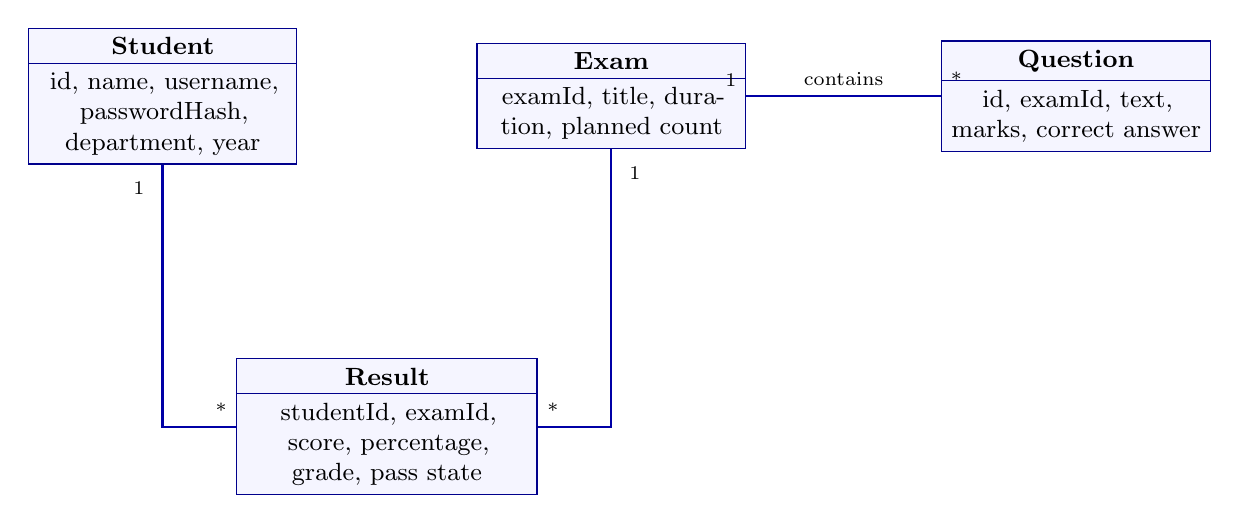
\begin{tikzpicture}
  \node[cls2,text width=32mm] (student) at (2.0,0) {\textbf{Student}\nodepart{second}id, name, username, passwordHash, department, year};
  \node[cls2,text width=32mm] (exam) at (7.7,0) {\textbf{Exam}\nodepart{second}examId, title, duration, planned count};
  \node[cls2,text width=32mm] (question) at (13.6,0) {\textbf{Question}\nodepart{second}id, examId, text, marks, correct answer};
  \node[cls2,text width=36mm] (result) at (4.85,-4.2) {\textbf{Result}\nodepart{second}studentId, examId, score, percentage, grade, pass state};
  \draw[thick,draw=blue!65!black] (exam.east) -- node[above,lbl]{contains} (question.west);
  \node[lbl,above left] at (exam.east) {1};
  \node[lbl,above right] at (question.west) {*};
  \draw[thick,draw=blue!65!black] (student.south) |- (result.west);
  \draw[thick,draw=blue!65!black] (exam.south) |- (result.east);
  \node[lbl] at ($(student.south)+(-0.3,-0.3)$) {1};
  \node[lbl] at ($(exam.south)+(0.3,-0.3)$) {1};
  \node[lbl,above left] at (result.west) {*};
  \node[lbl,above right] at (result.east) {*};
\end{tikzpicture}
\caption{Logical data model of the plain-text records.}
\label{fig:datamodel}
\end{figure}

\subsection{Sequence Diagram: Sign-in and Session}
Figure~\ref{fig:authseq} shows how a sign-in request becomes an in-memory session token.

\begin{figure}[H]
\centering
\hyphenpenalty=10000 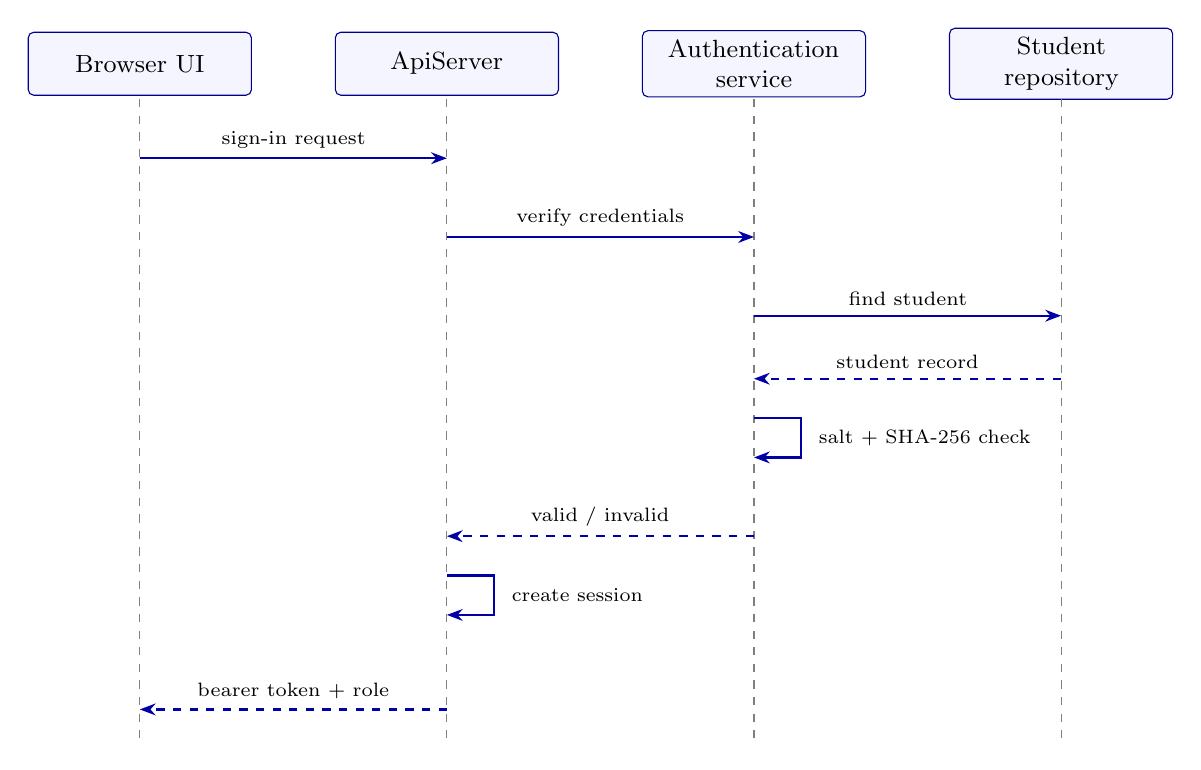
\begin{tikzpicture}
  \foreach \x/\t in {1.3/Browser UI,5.2/ApiServer,9.1/Authentication service,13.0/Student repository}{
    \node[uml,text width=26mm] at (\x,0) {\t};
    \draw[dashed,gray] (\x,-0.45) -- (\x,-8.6);}
  \msg{-1.2}{1.3}{5.2}{sign-in request}
  \msg{-2.2}{5.2}{9.1}{verify credentials}
  \msg{-3.2}{9.1}{13.0}{find student}
  \ret{-4.0}{13.0}{9.1}{student record}
  \selfmsg{-4.5}{9.1}{salt + SHA-256 check}
  \ret{-6.0}{9.1}{5.2}{valid / invalid}
  \selfmsg{-6.5}{5.2}{create session}
  \ret{-8.2}{5.2}{1.3}{bearer token + role}
\end{tikzpicture}
\caption{Authentication and session creation sequence.}
\label{fig:authseq}
\end{figure}

\subsection{Sequence Diagram: Exam and Question Management}
Figure~\ref{fig:adminseq} shows the administrator flow for creating an examination and adding a question.

\begin{figure}[H]
\centering
\hyphenpenalty=10000 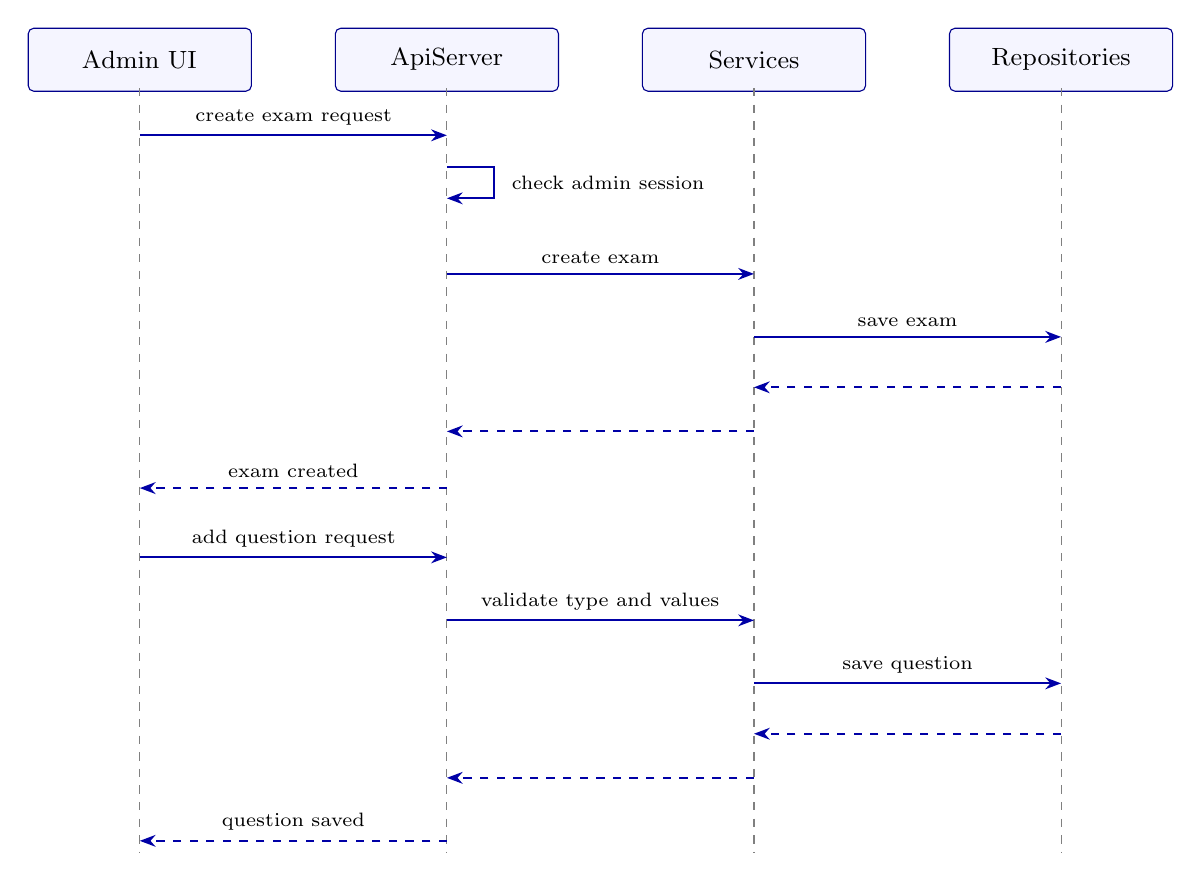
\begin{tikzpicture}[yscale=0.8]
  \foreach \x/\t in {1.3/Admin UI,5.2/ApiServer,9.1/Services,13.0/Repositories}{
    \node[uml,text width=26mm] at (\x,0) {\t};
    \draw[dashed,gray] (\x,-0.45) -- (\x,-12.6);}
  \msg{-1.2}{1.3}{5.2}{create exam request}
  \selfmsg{-1.7}{5.2}{check admin session}
  \msg{-3.4}{5.2}{9.1}{create exam}
  \msg{-4.4}{9.1}{13.0}{save exam}
  \ret{-5.2}{13.0}{9.1}{}
  \ret{-5.9}{9.1}{5.2}{}
  \ret{-6.8}{5.2}{1.3}{exam created}
  \msg{-7.9}{1.3}{5.2}{add question request}
  \msg{-8.9}{5.2}{9.1}{validate type and values}
  \msg{-9.9}{9.1}{13.0}{save question}
  \ret{-10.7}{13.0}{9.1}{}
  \ret{-11.4}{9.1}{5.2}{}
  \ret{-12.4}{5.2}{1.3}{question saved}
\end{tikzpicture}
\caption{Administrator sequence for exam creation and question authoring.}
\label{fig:adminseq}
\end{figure}

\section{Implementation Details}
\subsection{Authentication and Session Handling}
Student passwords are stored as a salt plus a SHA-256 digest in the user model implementation; plaintext is not stored. The web server creates in-memory bearer-token sessions after successful login and checks a session's role for protected endpoints. The administrator is initialized in server code with the demonstration credentials \texttt{admin} / \texttt{Admin@123}; this is a development default and should be changed before any real deployment. The custom SHA-256 password scheme is educational code and is not a production password-storage design; a maintained password-hashing function such as Argon2id or bcrypt with appropriate parameters should be used for real accounts.

\subsection{Timing, Evaluation, and Persistence}
In the console flow, the \texttt{Timer} measures elapsed time with \texttt{steady\_clock}. In the web flow, the server records attempt start times and calculates the remaining duration from that server-side time. The submission route applies a 15-second grace allowance for network delay. Result calculation is centralized in \texttt{EvaluationService}; the pass threshold in \texttt{Result} is 40 percent. The repositories store student, exam, question, and result records in separate text files, which keeps the prototype simple but means it is intended for small single-server demonstrations rather than concurrent multi-instance use.

\subsection{Screenshots}
The following screenshots were supplied with the project context. They are included as application evidence and are not substitutes for the TikZ-native diagrams above.

\begin{figure}[htbp]
\centering
\fbox{\includegraphics[width=0.96\textwidth]{screenshot-role-selection.png}}
\caption{ExamEra landing page with student and administrator entry paths.}
\label{fig:landing}
\end{figure}

\begin{figure}[htbp]
\centering
\fbox{\includegraphics[width=0.98\textwidth]{screenshot-student-dashboard.png}}
\caption{Student dashboard showing available examinations, scores, and recent results.}
\label{fig:student}
\end{figure}

\begin{figure}[htbp]
\centering
\fbox{\includegraphics[width=0.98\textwidth]{screenshot-admin-dashboard.png}}
\caption{Administrator examination overview with exam creation and attempt summaries.}
\label{fig:admin}
\end{figure}

\section{Limitations and Future Enhancements}
The supplied implementation uses local text files and in-memory server sessions. Data access is serialized with a process-local mutex, so multiple server instances do not share session or attempt state. The administrator demo credential is embedded in source, and the password hashing implementation is not suitable for production. The available question classes are MCQ and true/false. The project would benefit from a database-backed repository, configurable administrator accounts, a vetted password-hashing library, persistent session/attempt records, stronger deployment security, and automated test coverage.

\section{Conclusion}
The Online Examination System demonstrates a complete small-scale assessment workflow: role-aware entry, examination and question management, timed attempts, automatic grading, and result review. Its C++ domain model uses abstraction, inheritance, encapsulation, and runtime polymorphism, while services and repositories organize application logic and persistence. The web interface makes the flow accessible through a browser, and the supplied screenshots illustrate the student and administrator views. The existing implementation is appropriate as an OOP mini-project prototype, with the limitations above understood.

\end{document}